\documentclass[12pt, titlepage]{article}

\usepackage{fullpage}
\usepackage[round]{natbib}
\usepackage{multirow}
\usepackage{booktabs}
\usepackage{tabularx}
\usepackage{graphicx}
\usepackage{float}
\usepackage{hyperref}
\hypersetup{
    colorlinks,
    citecolor=blue,
    filecolor=black,
    linkcolor=red,
    urlcolor=blue
}

%% Comments

\usepackage{color}

\newif\ifcomments\commentstrue %displays comments
%\newif\ifcomments\commentsfalse %so that comments do not display

\ifcomments
\newcommand{\authornote}[3]{\textcolor{#1}{[#3 ---#2]}}
\newcommand{\todo}[1]{\textcolor{red}{[TODO: #1]}}
\else
\newcommand{\authornote}[3]{}
\newcommand{\todo}[1]{}
\fi

\newcommand{\wss}[1]{\authornote{blue}{SS}{#1}} 
\newcommand{\plt}[1]{\authornote{magenta}{TPLT}{#1}} %For explanation of the template
\newcommand{\an}[1]{\authornote{cyan}{Author}{#1}}

%% Common Parts

\newcommand{\progname}{Software Engineering} % PUT YOUR PROGRAM NAME HERE
\newcommand{\authname}{Team \#13, ARC
    \\ Avanish, Ahluwalia
    \\ Russell, Davidson
    \\ Rafey, Malik
    \\ Abdul, Zulfiqar} % AUTHOR NAMES                  

\usepackage{hyperref}
    \hypersetup{colorlinks=true, linkcolor=blue, citecolor=blue, filecolor=blue,
                urlcolor=blue, unicode=false}
    \urlstyle{same}
                                


\newcounter{acnum}
\newcommand{\actheacnum}{AC\theacnum}
\newcommand{\acref}[1]{AC\ref{#1}}

\newcounter{ucnum}
\newcommand{\uctheucnum}{UC\theucnum}
\newcommand{\uref}[1]{UC\ref{#1}}

\newcounter{mnum}
\newcommand{\mthemnum}{M\themnum}
\newcommand{\mref}[1]{M\ref{#1}}

\begin{document}

\title{Module Guide for \progname{}} 
\author{\authname}
\date{January 17, 2025}

\maketitle

\pagenumbering{roman}

\section{Revision History}

\begin{tabularx}{\textwidth}{p{3cm}p{2cm}X}
\toprule {\bf Date} & {\bf Version} & {\bf Notes}\\
\midrule
2025-01-17 & 1.0 & Initial Version\\
2025-03-26 & 1.1 & Fixed minor mistakes in the dates \\
\bottomrule
\end{tabularx}

\newpage

\section{Reference Material}

This section records information for easy reference.

\subsection{Abbreviations and Acronyms}

\renewcommand{\arraystretch}{1.2}
\begin{tabular}{l l} 
  \toprule		
  \textbf{symbol} & \textbf{description}\\
  \midrule 
  AC & Anticipated Change\\
  DAG & Directed Acyclic Graph \\
  M & Module \\
  MG & Module Guide \\
  OS & Operating System \\
  R & Requirement\\
  SC & Scientific Computing \\
  SRS & Software Requirements Specification\\
  \progname & Explanation of program name\\
  UC & Unlikely Change \\
  \bottomrule
\end{tabular}\\

\newpage

\tableofcontents

\listoftables

\listoffigures

\newpage

\pagenumbering{arabic}

\section{Introduction}

Decomposing a system into modules is a commonly accepted approach to developing
software.  A module is a work assignment for a programmer or programming
team~\citep{ParnasEtAl1984}.  We advocate a decomposition
based on the principle of information hiding~\citep{Parnas1972a}.  This
principle supports design for change, because the ``secrets'' that each module
hides represent likely future changes.  Design for change is valuable in SC,
where modifications are frequent, especially during initial development as the
solution space is explored.  

Our design follows the rules layed out by \citet{ParnasEtAl1984}, as follows:
\begin{itemize}
\item System details that are likely to change independently should be the
  secrets of separate modules.
\item Each data structure is implemented in only one module.
\item Any other program that requires information stored in a module's data
  structures must obtain it by calling access programs belonging to that module.
\end{itemize}

After completing the first stage of the design, the Software Requirements
Specification (SRS), the Module Guide (MG) is developed~\citep{ParnasEtAl1984}. The MG
specifies the modular structure of the system and is intended to allow both
designers and maintainers to easily identify the parts of the software.  The
potential readers of this document are as follows:

\begin{itemize}
\item New project members: This document can be a guide for a new project member
  to easily understand the overall structure and quickly find the
  relevant modules they are searching for.
\item Maintainers: The hierarchical structure of the module guide improves the
  maintainers' understanding when they need to make changes to the system. It is
  important for a maintainer to update the relevant sections of the document
  after changes have been made.
\item Designers: Once the module guide has been written, it can be used to
  check for consistency, feasibility, and flexibility. Designers can verify the
  system in various ways, such as consistency among modules, feasibility of the
  decomposition, and flexibility of the design.
\end{itemize}

The rest of the document is organized as follows. Section
\ref{SecChange} lists the anticipated and unlikely changes of the software
requirements. Section \ref{SecMH} summarizes the module decomposition that
was constructed according to the likely changes. Section \ref{SecConnection}
specifies the connections between the software requirements and the
modules. Section \ref{SecMD} gives a detailed description of the
modules. Section \ref{SecTM} includes two traceability matrices. One checks
the completeness of the design against the requirements provided in the SRS. The
other shows the relation between anticipated changes and the modules. Section
\ref{SecUse} describes the use relation between modules.

\section{Anticipated and Unlikely Changes} \label{SecChange}

This section lists possible changes to the system. According to the likeliness
of the change, the possible changes are classified into two
categories. Anticipated changes are listed in Section \ref{SecAchange}, and
unlikely changes are listed in Section \ref{SecUchange}.

\subsection{Anticipated Changes} \label{SecAchange}

Anticipated changes are the source of the information that is to be hidden
inside the modules. Ideally, changing one of the anticipated changes will only
require changing the one module that hides the associated decision. The approach
adapted here is called design for
change.

\begin{description}
\item[\refstepcounter{acnum} \actheacnum \label{acHardware}:] The supported hardware device platforms and versions.
\item[\refstepcounter{acnum} \actheacnum \label{acAPI}:] The API endpoints on the server.
\item[\refstepcounter{acnum} \actheacnum \label{acSettings}:] The supported in-app settings.
\item[\refstepcounter{acnum} \actheacnum \label{acTour}:] The tour creation workflow.
\item[\refstepcounter{acnum} \actheacnum \label{acObjectImport}:] The supported object files that can be imported to generate AR Objects.
\item[\refstepcounter{acnum} \actheacnum \label{acPerformance}:] The features available on different devices due to performance or hardware limitations.
\item[\refstepcounter{acnum} \actheacnum \label{acMaps}:] The provider of the maps/routing functionality
\item[\refstepcounter{acnum} \actheacnum \label{acRenderNumber}:] The algorithm used to determine which AR Objects should be rendered in the Realm Screen.
\item[\refstepcounter{acnum} \actheacnum \label{acRenderStyle}:] The render style of AR Objects (shaders/materials).
\item[\refstepcounter{acnum} \actheacnum \label{acInterfaces}:] The interface layout for all the screens.
\end{description}

\newpage

\subsection{Unlikely Changes} \label{SecUchange}

The module design should be as general as possible. However, a general system is
more complex. Sometimes this complexity is not necessary. Fixing some design
decisions at the system architecture stage can simplify the software design. If
these decision should later need to be changed, then many parts of the design
will potentially need to be modified. Hence, it is not intended that these
decisions will be changed.

\begin{description}
\item[\refstepcounter{ucnum} \uctheucnum \label{ucFormat}:] The file format of AR Objects (including metadata).
\item[\refstepcounter{ucnum} \uctheucnum \label{ucFormat}:] The account details associated with a user.
\item[\refstepcounter{ucnum} \uctheucnum \label{ucLoginProcedure}:] Changes in login procedure (sequence of events to be carried out for a successful login to the application)
\item[\refstepcounter{ucnum} \uctheucnum \label{ucFormat}:] The types of users (General and Organization).
\item[\refstepcounter{ucnum} \uctheucnum \label{ucEngine}:] The game engine used (Unity for rendering and platform support)
\end{description}

\section{Module Hierarchy} \label{SecMH}

This section provides an overview of the module design. Modules are summarized
in a hierarchy decomposed by secrets in Table \ref{TblMH}. The modules listed
below, which are leaves in the hierarchy tree, are the modules that will
actually be implemented.

\begin{description}
\item [\refstepcounter{mnum} \mthemnum \label{mHardware}:] Hardware Module
\item [\refstepcounter{mnum} \mthemnum \label{mTutorial}:] Tutorial Module
\item [\refstepcounter{mnum} \mthemnum \label{mInventory}:] Inventory Module
\item [\refstepcounter{mnum} \mthemnum \label{mSubRealm}:] Sub-Realm Module
\item [\refstepcounter{mnum} \mthemnum \label{mTouring}:] Touring Module
\item [\refstepcounter{mnum} \mthemnum \label{mTourList}:] Tour List Module
\item [\refstepcounter{mnum} \mthemnum \label{mTourManagement}:] Tour Management Module
\item [\refstepcounter{mnum} \mthemnum \label{mSettings}:] Settings Module
\item [\refstepcounter{mnum} \mthemnum \label{mHelp}:] Help Module
\item [\refstepcounter{mnum} \mthemnum \label{mFriends}:] Friends Module
\item [\refstepcounter{mnum} \mthemnum \label{mMaps}:] Maps Module
\item [\refstepcounter{mnum} \mthemnum \label{mRealm}:] Realm Interface Module
\item [\refstepcounter{mnum} \mthemnum \label{mImporter}:] Object Importer Module
\item [\refstepcounter{mnum} \mthemnum \label{mPlacement}:] Object Placement Module
\item [\refstepcounter{mnum} \mthemnum \label{mInteraction}:] Object Interaction Module
\item [\refstepcounter{mnum} \mthemnum \label{mRender}:] Object Render Module
\item [\refstepcounter{mnum} \mthemnum \label{mCollision}:] Collision Detection Module
\item [\refstepcounter{mnum} \mthemnum \label{mRA}:] Restricted Area Detection Module
\item [\refstepcounter{mnum} \mthemnum \label{mWeather}:] Weather Detection Module
\item [\refstepcounter{mnum} \mthemnum \label{mTourProx}:] Tour Proximity Detection Module
\item [\refstepcounter{mnum} \mthemnum \label{mNotifs}:] Notifications Module
\item [\refstepcounter{mnum} \mthemnum \label{mRESTAPI}:] REST API Connection Module
\item [\refstepcounter{mnum} \mthemnum \label{mLocalDB}:] Local Database Manager Module
\item [\refstepcounter{mnum} \mthemnum \label{mDataSync}:] Data Sync Module
\item [\refstepcounter{mnum} \mthemnum \label{mServerDB}:] Server Database Manager Module
\item [\refstepcounter{mnum} \mthemnum \label{mAuth}:] Authentication Module
\end{description}

\begin{table}[h!]
\centering
\begin{tabular}{p{0.3\textwidth} p{0.6\textwidth}}
\toprule
\textbf{Level 1} & \textbf{Level 2}\\
\midrule

{Hardware-Hiding Module} & Hardware Module\\
\midrule

\multirow{7}{0.3\textwidth}{Behaviour-Hiding Module} & Tutorial Module\\
& Inventory Module\\
& Sub-Realm Module\\
& Touring Module\\
& Tour List Module\\
& Tour Management Module\\
& Settings Module\\
& Help Module\\
& Friends Module\\ 
& Maps Module\\
& Realm Interface Module\\
& Object Importer Module\\
& Object Placement Module\\
& Object Interaction Module\\
& Object Render Module\\
& Collision Detection Module\\
& Restricted Area Detection Module\\
& Weather Detection Module\\
& Tour Proximity Detection Module\\
& Notifications Module\\
\midrule

\multirow{3}{0.3\textwidth}{Software Decision Module} & REST API Connection Module\\
& Local Database Manager Module\\
& Data Sync Module\\
& Server Database Manager Module\\
& Authentication Module\\
\bottomrule

\end{tabular}
\caption{Module Hierarchy}
\label{TblMH}
\end{table}

\newpage

\section{Connection Between Requirements and Design} \label{SecConnection}

The design of the system is intended to satisfy the requirements developed in
the SRS. In this stage, the system is decomposed into modules. The connection
between requirements and modules is listed in Table~\ref{TblRT}.


\section{Module Decomposition} \label{SecMD}

Modules are decomposed according to the principle of ``information hiding''
proposed by \citet{ParnasEtAl1984}. The \emph{Secrets} field in a module
decomposition is a brief statement of the design decision hidden by the
module. The \emph{Services} field specifies \emph{what} the module will do
without documenting \emph{how} to do it. For each module, a suggestion for the
implementing software is given under the \emph{Implemented By} title. If the
entry is \emph{OS}, this means that the module is provided by the operating
system or by standard programming language libraries.  \emph{\progname{}} means the
module will be implemented by the \progname{} software.

Only the leaf modules in the hierarchy have to be implemented. If a dash
(\emph{--}) is shown, this means that the module is not a leaf and will not have
to be implemented.

\subsection{Hardware Hiding Modules (\mref{mHardware})}

\begin{description}
\item[Secrets:] The data structure and algorithm used to implement the virtual hardware.
\item[Services:] Serves as a virtual hardware used by the rest of the system. This module provides the interface between the hardware and the software, allowing the system to display outputs or accept inputs.
\item[Implemented By:] OS
\end{description}

\subsubsection{Device Input/Output Module}

\begin{description}
\item[Secrets:] How data is collected from and sent to device sensors like the camera, GPS, or microphone.
\item[Services:] Provides a standard interface for capturing sensor input (e.g., photos, location data) and delivering it to the higher-level system modules.
\item[Implemented By:] OS
\end{description}

\subsection{Behaviour-Hiding Module}

\begin{description}
\item[Secrets:]The contents of the required behaviours.
\item[Services:]Includes programs that provide externally visible behaviour of
  the system as specified in the software requirements specification (SRS)
  documents. This module serves as a communication layer between the
  hardware-hiding module and the software decision module. The programs in this
  module will need to change if there are changes in the SRS.
\item[Implemented By:] REALM
\end{description}

% \item[Type of Module:] [Record, Library, Abstract Object, or Abstract Data Type]
  % [Information to include for leaf modules in the decomposition by secrets tree.]

\subsubsection{Tutorial Module (\mref{mTutorial})}

\begin{description}
\item[Secrets:]The format and structure of the tutorial.
\item[Services:]Provides an interactive tutorial for a user to experiment with the core features of the app. The tutorial for individual features are also accessible.
\item[Implemented By:]REALM
\item[Type of Module:]Abstract Object
\end{description}

\subsubsection{Inventory Module (\mref{mInventory})}

\begin{description}
\item[Secrets:]The format and structure of the inventory interface.
\item[Services:]Display's a list of available objects and allows for detailed previews of AR Objects and their associated metadata.
\item[Implemented By:]REALM
\item[Type of Module:]Abstract Object
\end{description}

\subsubsection{Sub-Realm Module (\mref{mSubRealm})}

\begin{description}
\item[Secrets:]The format and structure of the Sub-Realms.
\item[Services:]Allows users to join and leave custom environments with controlled access management. Users with adequate permissions in a Sub-Realm can invite or remove other users. The default Sub-Realm is common between all users.
\item[Implemented By:]REALM
\item[Type of Module:]Abstract Object
\end{description}

\subsubsection{Touring Module (\mref{mTouring})}

\begin{description}
\item[Secrets:]The format and structure of touring.
\item[Services:]Allows \textit{General Users} to go on pre-made and geo-anchored tours by following a defined path that has AR objects placed along the route. Users can view the tours through the Realm Interface and Map views.
\item[Implemented By:]REALM
\item[Type of Module:]Abstract Object
\end{description}

\subsubsection{Tour List Module (\mref{mTourList})}

\begin{description}
\item[Secrets:]The format and structure of the tour list.
\item[Services:]Display's a list of available tours and allows a user to view more details about a specific tour.
\item[Implemented By:]REALM
\item[Type of Module:]Abstract Object
\end{description}

\subsubsection{Tour Management Module (\mref{mTourManagement})}

\begin{description}
\item[Secrets:]The format and structure of tour management.
\item[Services:]Display's a list of available tours and allows a user to view more details about a specific tour.
\item[Implemented By:]REALM
\item[Type of Module:]Abstract Object
\end{description}

\subsubsection{Settings Module (\mref{mSettings})}

\begin{description}
\item[Secrets:]The format and structure of settings.
\item[Services:]Gives users the option to customize their experience and accommodate disabilities.
\item[Implemented By:]REALM
\item[Type of Module:]Abstract Object
\end{description}

\subsubsection{Help Module (\mref{mHelp})}

\begin{description}
\item[Secrets:]The format and structure of the help page.
\item[Services:]Aides the user in understanding specific features or report issues within the app. The tutorial can also be launched from this module.
\item[Implemented By:]REALM
\item[Type of Module:]Abstract Object
\end{description}

\subsubsection{Friends Module (\mref{mFriends})}

\begin{description}
\item[Secrets:]The format and structure of the friends functionality.
\item[Services:]Allows users to manage their friends. These friends can be added to Sub-Realms with the right permissions.
\item[Implemented By:]REALM
\item[Type of Module:]Abstract Object
\end{description}

\subsubsection{Maps Module (\mref{mMaps})}

\begin{description}
\item[Secrets:]The format and structure of maps.
\item[Services:]Display's AR object locations superimposed on a 2D map of the area around the user. User can zoom in and out to see less or more objects.
\item[Implemented By:]REALM
\item[Type of Module:]Abstract Object
\end{description}

\subsubsection{Realm Interface Module (\mref{mRealm})}

\begin{description}
\item[Secrets:]The structure and interaction of the Realm Interface.
\item[Services:]This is the primary interface that the user interacts with to start the placement or interaction with AR Objects and switch between Sub-Realms.
\item[Implemented By:]REALM
\item[Type of Module:]Abstract Object
\end{description}

\subsubsection{Object Importer Module (\mref{mImporter})}

\begin{description}
\item[Secrets:]The structure and workflow of object importing.
\item[Services:]Scans of objects from external apps can be imported and turned into AR objects with the required additional metadata.
\item[Implemented By:]REALM
\item[Type of Module:]Abstract Object
\end{description}

\subsubsection{Object Placement Module (\mref{mPlacement})}

\begin{description}
\item[Secrets:]The structure and workflow of object placement.
\item[Services:]Allows a user to place an AR object in the world. The placement can be fine tuned after the initial location is selected.
\item[Implemented By:]REALM
\item[Type of Module:]Abstract Object
\end{description}

\subsubsection{Object Interaction Module (\mref{mInteraction})}

\begin{description}
\item[Secrets:]The structure and workflow of object interaction.
\item[Services:]Allows users to interact with existing AR objects in the world. They can add reactions, report, or save the objects to their inventory.
\item[Implemented By:]REALM
\item[Type of Module:]Abstract Object
\end{description}

\subsubsection{Object Render Module (\mref{mRender})}

\begin{description}
\item[Secrets:]The format and algorithm used to render AR objects.
\item[Services:]Balances the performance with the number and resolution of AR objects to ensure a fluid user experience.
\item[Implemented By:]REALM
\item[Type of Module:]Abstract Object
\end{description}

\subsubsection{Collision Detection Module (\mref{mCollision})}

\begin{description}
\item[Secrets:]The format and algorithm to achieve collision detection.
\item[Services:]Uses device sensor data to detect when a user is close to a physical object and warn them to prevent a possible collision.
\item[Implemented By:]REALM
\item[Type of Module:]Abstract Object
\end{description}

\subsubsection{Restricted Area Detection Module (\mref{mRA})}

\begin{description}
\item[Secrets:]The format and algorithm to achieve restricted area detection.
\item[Services:]Display's places on the map where access to a certain area is restricted.
\item[Implemented By:]REALM
\item[Type of Module:]Abstract Object
\end{description}

\subsubsection{Weather Detection Module (\mref{mWeather})}

\begin{description}
\item[Secrets:]The format and algorithm to achieve weather detection.
\item[Services:]Display's warnings for inclement weather in the area of the user.
\item[Implemented By:]REALM
\item[Type of Module:]Abstract Object
\end{description}

\subsubsection{Tour Proximity Detection Module (\mref{mTourProx})}

\begin{description}
\item[Secrets:]The format and algorithm to achieve tour proximity detection.
\item[Services:]Monitors the user's location to find when they are in close proximity to a tour.
\item[Implemented By:]REALM
\item[Type of Module:]Abstract Object
\end{description}

\subsubsection{Notifications Module (\mref{mNotifs})}

\begin{description}
\item[Secrets:]The structure and format of notifications.
\item[Services:]Sends notifications to the device if enabled.
\item[Implemented By:]REALM
\item[Type of Module:]Abstract Object
\end{description}

\subsection{Software Decision Module}

\begin{description}
\item[Secrets:] The design decision based on mathematical theorems, physical
  facts, or programming considerations. The secrets of this module are
  \emph{not} described in the SRS.
\item[Services:] Includes data structure and algorithms used in the system that
  do not provide direct interaction with the user. 
  % Changes in these modules are more likely to be motivated by a desire to
  % improve performance than by externally imposed changes.
\item[Implemented By:] REALM
\end{description}

\subsubsection{REST API Connection Module (\mref{mRESTAPI})}

\begin{description}
\item[Secrets:]The structure and format of the connection to the server REST API.
\item[Services:]Makes calls to and from the REST API running on the server.
\item[Implemented By:]REALM
\item[Type of Module:]Abstract Object
\end{description}

\subsubsection{Local Database Manager Module (\mref{mLocalDB})}

\begin{description}
\item[Secrets:]The structure and format of the local database interface.
\item[Services:]Interacts with the local database by performing CRUD operations.
\item[Implemented By:]REALM
\item[Type of Module:]Record
\end{description}

\subsubsection{Data Sync Module (\mref{mDataSync})}

\begin{description}
\item[Secrets:]The structure and algorithm to sync data.
\item[Services:]Keeps the local app data and server data in sync. 
\item[Implemented By:]REALM
\item[Type of Module:]Abstract Object
\end{description}

\subsubsection{Server Database Manager Module (\mref{mServerDB})}

\begin{description}
\item[Secrets:]The structure and format of the server database interface.
\item[Services:]Interacts with the server database by performing CRUD operations.
\item[Implemented By:]REALM
\item[Type of Module:]Record
\end{description}

\subsubsection{Authentication Module (\mref{mAuth})}

\begin{description}
\item[Secrets:]The structure and format of the authentication.
\item[Services:]Verifies a user's credentials and which type of user they are (General/Organization user).
\item[Implemented By:]REALM
\item[Type of Module:]Abstract Object
\end{description}

\newpage

\section{Traceability Matrix} \label{SecTM}

This section shows two traceability matrices: between the modules and the
requirements and between the modules and the anticipated changes.

% the table should use mref, the requirements should be named, use something
% like fref
\begin{table}[H]
\centering
\begin{tabular}{p{0.2\textwidth} p{0.6\textwidth}}
\toprule
\textbf{Req.} & \textbf{Modules}\\
\midrule
EI-LF1 & \mref{mRealm}\\
MP-FR1 & \mref{mMaps}\\
MP-FR2 & \mref{mMaps}, \mref{mRESTAPI}\\
MP-FR3 & \mref{mMaps}\\
MP-FR4 & \mref{mMaps}\\
MP-FR5 & \mref{mMaps}, \mref{mSubRealm}\\
MP-FR6 & \mref{mMaps}\\
MP-FR7 & \mref{mMaps}\\
MP-FR8 & \mref{mMaps}\\
MP-FR9 & \mref{mMaps}\\
MP-FR10 & \mref{mMaps}, \mref{mRA}\\
IV-FR1 & \mref{mInventory}, \mref{mRESTAPI}\\
IV-FR2 & \mref{mInventory}, \mref{mRESTAPI}, \mref{mImporter}, \mref{mInteraction}\\
IV-FR3 & \mref{mInventory}\\
IV-FR4 & \mref{mInventory}\\
IV-FR5 & \mref{mInventory}, \mref{mRESTAPI}, \mref{mImporter}, \mref{mInteraction}\\
IV-FR6 & \mref{mInventory}\\
IV-FR7 & \mref{mInventory}\\
IV-FR8 & \mref{mInventory}\\
IV-FR9 & \mref{mInventory}\\
IV-FR10 & \mref{mInventory}\\
IV-FR11 & \mref{mInventory}, \mref{mSettings}\\
\bottomrule
\end{tabular}
\caption{Trace Between Requirements and Modules}
\label{TblRT}
\end{table}

\begin{table}[H]
\centering
\begin{tabular}{p{0.2\textwidth} p{0.6\textwidth}}
\toprule
\textbf{Req.} & \textbf{Modules}\\
\midrule
OUI-FR1 & \mref{mImporter}\\
OUI-FR2 & \mref{mImporter}\\
OUI-FR3 & \mref{mImporter}\\
OUI-FR4 & \mref{mImporter}, \mref{mRESTAPI}\\ 
OUI-FR5 & \mref{mImporter}\\
OUI-FR6 & \mref{mImporter}\\
OUI-FR7 & \mref{mImporter}, \mref{mRESTAPI}\\
OUI-FR8 & \mref{mImporter}, \mref{mRESTAPI}\\
OUI-FR9 & \mref{mImporter}, \mref{mRESTAPI}\\
OUI-FR10 & \mref{mImporter}, \mref{mRESTAPI}\\
OUI-FR11 & \mref{mImporter}, \mref{mRESTAPI}\\
OUI-FR12 & \mref{mImporter}\\
TU-FR1 & \mref{mTutorial}\\
TU-FR2 & \mref{mTutorial}\\
TU-FR3 & \mref{mTutorial}\\
TU-FR4 & \mref{mTutorial}, \mref{mSettings}\\
TU-FR5 & \mref{mTutorial}\\
TM-FR1 & \mref{mTourManagement}, \mref{mAuth}\\
TM-FR2 & \mref{mTourManagement}, \mref{mRESTAPI}, \mref{mAuth}\\
TM-FR3 & \mref{mTourManagement}, \mref{mRESTAPI}\\
TM-FR4 & \mref{mTourManagement}, \mref{mAuth}\\
TM-FR5 & \mref{mTourManagement}, \mref{mAuth}\\
TM-FR6 & \mref{mTourManagement}, \mref{mRESTAPI}, \mref{mAuth}\\
TR-FR1 & \mref{mTouring}, \mref{mAuth}\\
TR-FR2 & \mref{mTouring}, \mref{mAuth}, \mref{mTourList} \mref{mTourProx}, \mref{mNotifs}\\
TR-FR3 & \mref{mTouring}\\
TR-FR4 & \mref{mTouring}, \mref{mMaps}, \mref{mRealm}\\
OP-FR1 & \mref{mPlacement}, \mref{mRESTAPI}, \mref{mSubRealm}\\
OP-FR2 & \mref{mPlacement}, \mref{mRESTAPI}, \mref{mSubRealm}\\
OP-FR3 & \mref{mPlacement}\\
OP-FR4 & \mref{mPlacement}, \mref{mRESTAPI}\\
\bottomrule
\end{tabular}
\caption{(Cont.) Trace Between Requirements and Modules}
\label{TblRT}
\end{table}

\begin{table}[H]
\centering
\begin{tabular}{p{0.2\textwidth} p{0.6\textwidth}}
\toprule
\textbf{Req.} & \textbf{Modules}\\
\midrule
RI-FR1 & \mref{mRealm}, \mref{mHardware}\\
RI-FR2 & \mref{mRealm}, \mref{mSubRealm}\\
RI-FR3 & \mref{mRealm}, \mref{mPlacement}\\
RI-FR4 & \mref{mRealm}, \mref{mImporter}\\
RI-FR5 & \mref{mRealm}, \mref{mTourManagement}\\
RI-FR6 & \mref{mRealm}, \mref{mWeather}\\
RI-FR7 & \mref{mRealm}, \mref{mCollision}\\
RI-FR8 & \mref{mRealm}, \mref{mLocalDB}, \mref{mDataSync}\\
AI-FR1 & \mref{mAuth}\\
AI-FR2 & \mref{mAuth}, \mref{mRESTAPI}\\
PS-FR1 & \mref{mAuth}, \mref{mRESTAPI}\\
PS-FR2 & \mref{mAuth}, \mref{mRESTAPI}\\
PS-FR3 & \mref{mAuth}, \mref{mRESTAPI}\\
PS-FR4 & \mref{mAuth}, \mref{mRESTAPI}\\
PS-FR5 & \mref{mAuth}, \mref{mSubRealm}\\
PS-FR6 & \mref{mAuth}, \mref{mHelp}\\
G-FR1 & \mref{mSubRealm}, \mref{mRESTAPI}\\
G-FR2 & \mref{mSubRealm}, \mref{mRESTAPI}\\
G-FR3 & \mref{mSubRealm}, \mref{mRESTAPI}\\
G-FR4 & \mref{mSubRealm}, \mref{mRESTAPI}\\
G-FR5 & \mref{mSubRealm}, \mref{mRESTAPI}\\
FS-FR1 & \mref{mFriends}, \mref{mRESTAPI}\\
FS-FR2 & \mref{mFriends}, \mref{mRESTAPI}\\
FS-FR3 & \mref{mFriends}, \mref{mRESTAPI}\\
FS-FR4 & \mref{mFriends}, \mref{mRESTAPI}\\
S-FR1 & \mref{mSettings}, \mref{mLocalDB}\\
S-FR2 & \mref{mSettings}, \mref{mLocalDB}\\
S-FR3 & \mref{mSettings}, \mref{mRESTAPI}\\
S-FR4 & \mref{mSettings}, \mref{mRESTAPI}\\
S-FR5 & \mref{mSettings}, \mref{mRESTAPI}, \mref{mSubRealm}\\
S-FR6 & \mref{mSettings}, \mref{mLocalDB}\\
DB-FR1 & \mref{mLocalDB}, \mref{mServerDB}, \mref{mDataSync}\\
DB-FR2 & \mref{mLocalDB}, \mref{mServerDB}, \mref{mDataSync}\\
\bottomrule
\end{tabular}
\caption{(Cont.) Trace Between Requirements and Modules}
\label{TblRT}
\end{table}

\begin{table}[H]
\centering
\begin{tabular}{p{0.2\textwidth} p{0.6\textwidth}}
\toprule
\textbf{Req.} & \textbf{Modules}\\
\midrule
QS-P1 & \mref{mMaps}\\
QS-P2 & \mref{mInventory}\\
QS-P3 & \mref{mRender}\\
QS-P4 & \mref{mImporter}\\
QS-P5 & \mref{mRender}\\
QS-U1 & \mref{mSettings}\\
QS-U2 & \textit{All}\\
QS-SC1 & \mref{mLocalDB}, \mref{mServerDB}, \mref{mDataSync}\\
QS-SC2 & \mref{mLocalDB}, \mref{mServerDB}, \mref{mDataSync}\\
QS-SA1 & \mref{mRealm}, \mref{mRender}, \mref{mCollision}, \mref{mRA}\\
QS-SA2 & \mref{mRealm}, \mref{mRender}, \mref{mCollision}, \mref{mRA}\\
QS-R1 & \mref{mLocalDB}, \mref{mServerDB}\\
QS-A1 & \mref{mLocalDB}, \mref{mServerDB}\\
DI-I1 & \mref{mHardware}\\
DI-I2 & \mref{mHardware}\\
DI-D1 & \mref{mHardware}\\
DI-D2 & \mref{mHardware}\\
DI-D3 & \mref{mHardware}\\
DI-D4 & \mref{mHardware}\\
DI-M1 & \mref{mRESTAPI}\\
DI-R1 & \mref{mInventory}, \mref{mSubRealm}, \mref{mTouring}, \mref{mTourManagement}, \mref{mSettings}, \mref{mHelp}, \mref{mHelp}, \mref{mFriends}, \mref{mRealm}, \mref{mMaps}, \mref{mImporter}, \mref{mPlacement}, \mref{mInteraction}\\
DI-P1 & \mref{mHardware}\\
DI-P2 & \mref{mHardware}\\
\bottomrule
\end{tabular}
\caption{(Cont.) Trace Between Requirements and Modules}
\label{TblRT}
\end{table}

\begin{table}[H]
\centering
\begin{tabular}{p{0.2\textwidth} p{0.6\textwidth}}
\toprule
\textbf{AC} & \textbf{Modules}\\
\midrule
\acref{acHardware} & \mref{mHardware}\\
\acref{acAPI} & \mref{mDataSync}, \mref{mRESTAPI}\\
\acref{acSettings} & \mref{mSettings}\\
\acref{acTour} & \mref{mTourManagement}\\
\acref{acObjectImport} & \mref{mHardware}, \mref{mImporter}\\
\acref{acPerformance} & \mref{mHardware}\\
\acref{acMaps} & \mref{mMaps}\\
\acref{acRenderNumber} & \mref{mRender}\\
\acref{acRenderStyle} & \mref{mRender}\\
\acref{acInterfaces} & \mref{mInventory}, \mref{mSubRealm}, \mref{mTouring}, \mref{mTourManagement}, \mref{mSettings}, \mref{mHelp}, \mref{mHelp}, \mref{mFriends}, \mref{mRealm}, \mref{mMaps}, \mref{mImporter}, \mref{mPlacement}, \mref{mInteraction}\\
\bottomrule
\end{tabular}
\caption{Trace Between Anticipated Changes and Modules}
\label{TblACT}
\end{table}

\newpage

\section{Use Hierarchy Between Modules} \label{SecUse}

In this section, the uses hierarchy between modules is
provided. \citet{Parnas1978} said of two programs A and B that A {\em uses} B if
correct execution of B may be necessary for A to complete the task described in
its specification. That is, A {\em uses} B if there exist situations in which
the correct functioning of A depends upon the availability of a correct
implementation of B.  Figure \ref{FigUH} illustrates the use relation between
the modules. It can be seen that the graph is a directed acyclic graph
(DAG). Each level of the hierarchy offers a testable and usable subset of the
system, and modules in the higher level of the hierarchy are essentially simpler
because they use modules from the lower levels.

\begin{figure}[H]
\centering
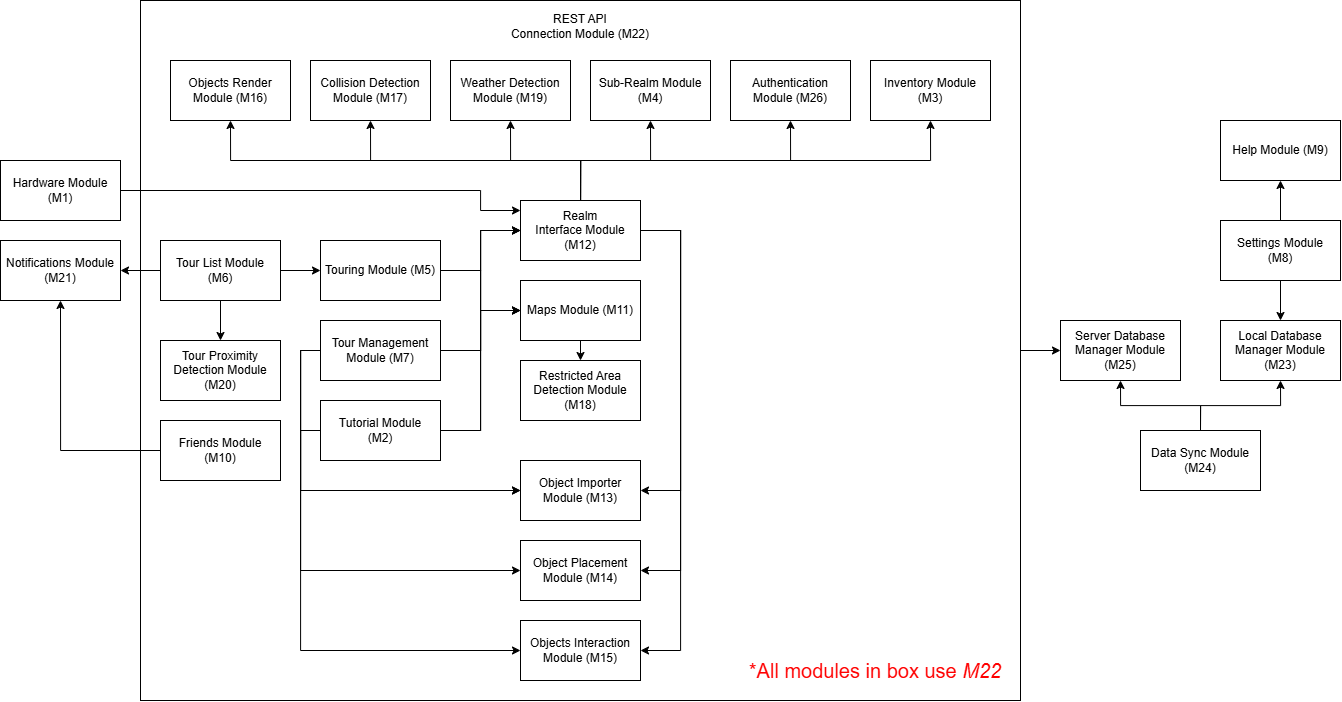
\includegraphics[width=1\textwidth]{UsesHierarchy.png}
\caption{Use hierarchy among modules}
\label{FigUH}
\end{figure}

%\section*{References}

\section{User Interfaces}

The following are images of various major interfaces:

\begin{figure}[H]
\centering
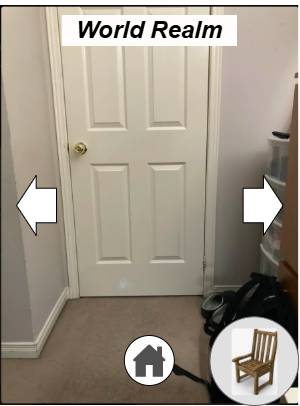
\includegraphics[width=0.7\textwidth]{RIScreen.png}
\caption{Realm Interface Screen}
\label{FigRI}
\end{figure}

\begin{figure}[H]
\centering
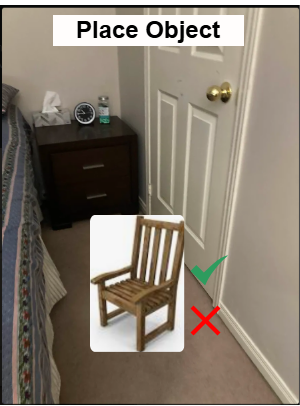
\includegraphics[width=0.7\textwidth]{OPScreen.png}
\caption{Object Placement Screen}
\label{FigOP}
\end{figure}

\begin{figure}[H]
\centering
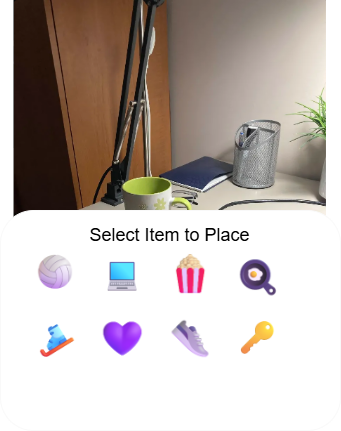
\includegraphics[width=0.7\textwidth]{IScreen.png}
\caption{Inventory Screen}
\label{FigI}
\end{figure}

\section{Design of Communication Protocols}

N/A

\section{Timeline}
Below is a schedule for our implementation and work distribution of the modules.

\begin{table}[H]
\begin{tabular}{lll}
\hline
\multicolumn{1}{|l|}{\textbf{Due Date}}                & \multicolumn{1}{l|}{\textbf{Work to be Completed}}            & \multicolumn{1}{l|}{\textbf{Assigned Member}} \\ \hline
\multicolumn{1}{|l|}{\multirow{3}{*}{Jan 15 - Jan 20}} & \multicolumn{1}{l|}{Hardware Module}                          & \multicolumn{1}{l|}{Avanish}                  \\ \cline{2-3} 
\multicolumn{1}{|l|}{}                                 & \multicolumn{1}{l|}{Tutorial Module}                          & \multicolumn{1}{l|}{Russell}                  \\ \cline{2-3} 
\multicolumn{1}{|l|}{}                                 & \multicolumn{1}{l|}{Inventory Module}                         & \multicolumn{1}{l|}{Avanish}                  \\ \hline
\multicolumn{1}{|l|}{\multirow{4}{*}{Jan 20 - Jan 25}} & \multicolumn{1}{l|}{Sub-Realm Module}                         & \multicolumn{1}{l|}{Abdul}                    \\ \cline{2-3} 
\multicolumn{1}{|l|}{}                                 & \multicolumn{1}{l|}{Touring Module}                           & \multicolumn{1}{l|}{Russell}                  \\ \cline{2-3} 
\multicolumn{1}{|l|}{}                                 & \multicolumn{1}{l|}{Tour List Module}                         & \multicolumn{1}{l|}{Russell}                  \\ \cline{2-3} 
\multicolumn{1}{|l|}{}                                 & \multicolumn{1}{l|}{Tour Management Module}                   & \multicolumn{1}{l|}{Russell}                  \\ \hline
\multicolumn{1}{|l|}{\multirow{4}{*}{Jan 25 - Feb 1}}  & \multicolumn{1}{l|}{Settings Module}                          & \multicolumn{1}{l|}{Rafey}                    \\ \cline{2-3} 
\multicolumn{1}{|l|}{}                                 & \multicolumn{1}{l|}{Help Module}                              & \multicolumn{1}{l|}{Rafey}                    \\ \cline{2-3} 
\multicolumn{1}{|l|}{}                                 & \multicolumn{1}{l|}{Friends Module}                           & \multicolumn{1}{l|}{Rafey}                    \\ \cline{2-3} 
\multicolumn{1}{|l|}{}                                 & \multicolumn{1}{l|}{Maps Module}                              & \multicolumn{1}{l|}{Abdul}                    \\ \hline
\multicolumn{1}{|l|}{\multirow{5}{*}{Jan 30 - Feb 5}}  & \multicolumn{1}{l|}{Realm Interface Module}                   & \multicolumn{1}{l|}{Russell}                  \\ \cline{2-3} 
\multicolumn{1}{|l|}{}                                 & \multicolumn{1}{l|}{Object Importer Module}                   & \multicolumn{1}{l|}{Abdul}                    \\ \cline{2-3} 
\multicolumn{1}{|l|}{}                                 & \multicolumn{1}{l|}{Object Placement Module}                  & \multicolumn{1}{l|}{Avanish}                  \\ \cline{2-3} 
\multicolumn{1}{|l|}{}                                 & \multicolumn{1}{l|}{Object Interaction Module}                & \multicolumn{1}{l|}{Abdul}                    \\ \cline{2-3} 
\multicolumn{1}{|l|}{}                                 & \multicolumn{1}{l|}{Object Render Module}                     & \multicolumn{1}{l|}{Abdul}                    \\ \hline
\multicolumn{1}{|l|}{\multirow{4}{*}{Feb 5 - Feb 10}}  & \multicolumn{1}{l|}{Collision Hazard Detection Module}         & \multicolumn{1}{l|}{Rafey}                    \\ \cline{2-3} 
\multicolumn{1}{|l|}{}                                 & \multicolumn{1}{l|}{Restricted Area Detection Module}          & \multicolumn{1}{l|}{Avanish}                  \\ \cline{2-3} 
\multicolumn{1}{|l|}{}                                 & \multicolumn{1}{l|}{Weather Hazard Detection Module}           & \multicolumn{1}{l|}{Avanish}                  \\ \cline{2-3} 
\multicolumn{1}{|l|}{}                                 & \multicolumn{1}{l|}{Tour Proximity Detection Module}           & \multicolumn{1}{l|}{Rafey}                    \\ \hline
\multicolumn{1}{|l|}{\multirow{4}{*}{Feb 6 - Feb 10}}  & \multicolumn{1}{l|}{Notifications Module}                     & \multicolumn{1}{l|}{Rafey}                    \\ \cline{2-3} 
\multicolumn{1}{|l|}{}                                 & \multicolumn{1}{l|}{REST API Module}                          & \multicolumn{1}{l|}{Abdul}                    \\ \cline{2-3} 
\multicolumn{1}{|l|}{}                                 & \multicolumn{1}{l|}{Local Database Manager Module}             & \multicolumn{1}{l|}{Abdul}                    \\ \cline{2-3} 
\multicolumn{1}{|l|}{}                                 & \multicolumn{1}{l|}{Data Sync Module}                         & \multicolumn{1}{l|}{Russell}                  \\ \hline
\multicolumn{1}{|l|}{\multirow{2}{*}{Feb 8 - Feb 10}}  & \multicolumn{1}{l|}{Server Database Manager Module}            & \multicolumn{1}{l|}{Abdul}                    \\ \cline{2-3} 
\multicolumn{1}{|l|}{}                                 & \multicolumn{1}{l|}{Authentication Module}                    & \multicolumn{1}{l|}{Rafey}                    \\ \hline
                                                       &                                                                &                                              
\end{tabular}
\caption{Module Development Schedule}
\label{tab:module_schedule}
\end{table}

\bibliographystyle {plainnat}
\bibliography{../../../refs/References}

\newpage{}

\end{document}